\documentclass{report}
\usepackage[utf8]{inputenc}
\usepackage{graphicx}
\usepackage{hyperref}
\usepackage[a4paper, margin=1in]{geometry}

\title{\textbf{ASSR: Automatic Stuttered Speech Recognition}}
\author{Anshul Gupta (16305R001) \\ Kapil Aggarwal (16305R010)}
\date{\today}

\begin{document}

\maketitle

\tableofcontents

\chapter{Introduction}
More than 70 million people worldwide are stutterers -- that's one in every 100.

Past few years have seen an increase in popularity of personal voice assistants which can actually speed up the day to day tasks. But that is limited by the ability of the speaker.
If the input to the voice recognition system is from a stutterer, it fails miserably with accuracy as low as 18\% and as high as 73\% as compared to a baseline of 92\% for normal speaker \cite{siriStats}. So our project aims to correct the Speech-to-Text conversion for a stuttered speech.

The existing work \cite{manuChopra} that has been done for this problem is just classification of a speech as a stuttered speech or a normal speech. The approach they use is pre-emphasis of audio and then extract audio features (most of the models used MFCC features) and training the classifier models (ANNs, HMMs, SVMs etc.)
In one literature, they use RMS, standard mean, median frequency, peak to peak analysis (the difference between the highest and the lowest frequency peaks in a .wav file) and a specialized mean feature extractor as the features for training the ANN.


\chapter{Dataset}
One of the challenges for this project was to get a time-aligned labelled dataset.

The dataset we are using is University College London Archive of Stuttered Speech (UCLASS) \cite{uclass}. It contains recordings of monologues, reading and conversations of different speakers ranging from 7 years old to 20 years old. Unfortunately, most of the recordings do not have orthographic transcriptions and/or time aligned transcriptions. The database has audio files in 2 releases, release 1 and release 2. Release 1 has 16 files which have time-aligned transcriptions and release 2 has only 4 files which have time-aligned transcriptions. So we worked with the 16 files from release 1 to train our models. 

The audio files are in .wav format having a sampling rate of 22050Hz and the corresponding time-aligned transcriptions are in CHILDES CHAT \cite{childes} format. The orthographic transcriptions are in plain text.

Also the orthographic transcriptions do not have the text for the corrected speech. It has the transcription for the stuttered speech. So we had to manually transcribe the the audio files.

\chapter{Methodology and Implementation Details}

\begin{figure}[ht]
    \centering
    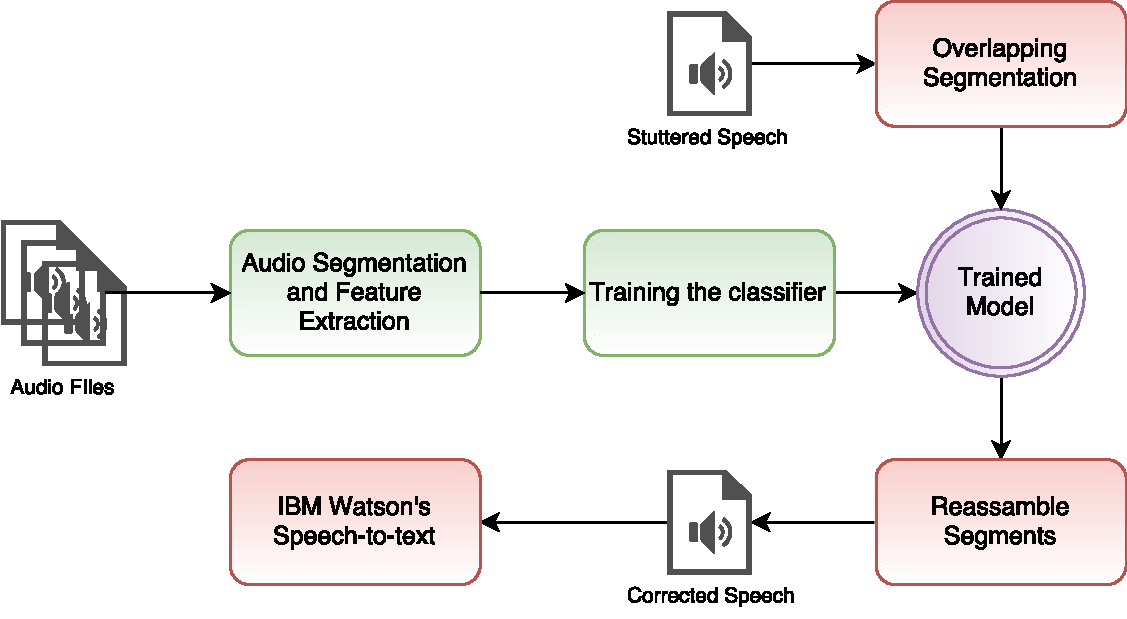
\includegraphics[scale=0.70]{FlowDiagram.pdf}
    \caption{Flow Diagram}
    \label{fig:flowdiagram}
\end{figure}

\section{Data Processing}
\subsection{Data Pre-Processing}
We used the time-aligned transcriptions to split the data files into stuttered segments and normal segments. The transcriptions had the start time and end time (in milliseconds) for each segment. So there were in all 12,633 segments that we got after splitting the audio files.

\begin{table}[ht]
\centering
\caption{Data Statistics}
\label{table:data-statistics}
\begin{tabular}{|l|r|r|r|}
\hline
                     & \multicolumn{1}{l|}{\textbf{ALL}} & \multicolumn{1}{l|}{\textbf{STUTTER}} & \multicolumn{1}{l|}{\textbf{NORMAL}} \\ \hline
\textbf{COUNT}       & 12633                             & 2643                                  & 9990                                 \\ \hline
\textbf{MAX (ms)}    & 17044                             & 17044                                 & 14499                                \\ \hline
\textbf{MIN (ms)}    & 0                                 & 1                                     & 0                                    \\ \hline
\textbf{MEAN (ms)}   & 315.0925                          & 762.5323                              & 196.7158                             \\ \hline
\textbf{MEDIAN (ms)} & 192                               & 486                                   & 168                                  \\ \hline
\textbf{MODE (ms)}   & 109                               & 201                                   & 93                                   \\ \hline
\end{tabular}
\end{table}

From Table \ref{table:data-statistics} we can see that the average duration of all the segments is $\sim$ 315 ms and stuttered segments are about 2.5 times longer than the average segment and the longest stutter was around 17 seconds. Training the data on such skewed data will not be useful because seeing a stuttered segment as long as 17 seconds is very unlikely.

So, instead of using the segments of variable duration, we segmented the files segments further down to less than or equal to 300 ms (figure \ref{fig:audioSegments}) which is close to the average length of the segments. This segmentation created 17,545 segments which were used for training the models.

\begin{figure}[ht]
    \centering
    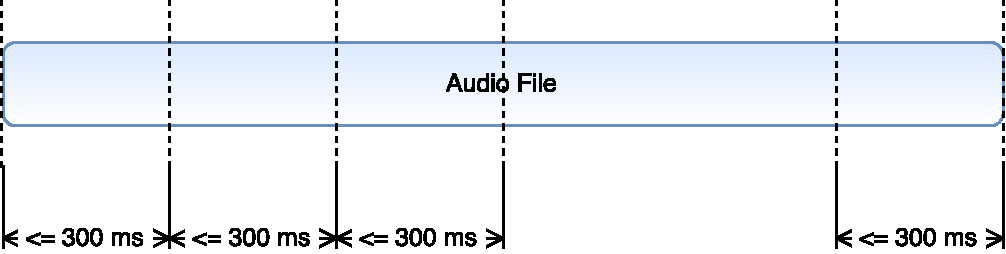
\includegraphics[scale=0.7]{AudioSplits300ms.pdf}
    \caption{Audio segments}
    \label{fig:audioSegments}
\end{figure}

\subsection{Feature Extraction}
Once the audio segments were prepared, we then extracted the features from each segments which can be fed to the classification models.

We used MFCC features as they are very representative of human speech and RMSE which represents the loudness of a speech. We extracted 39 MFCC features and RMSE for each segment and stored the mean and variance of all 40 features (39 MFCC + 1 RMSE) to get a feature vector of 80 components.

In the end, our dataset had 17,545 rows each having 80 features.

\section{Classification}
Now with the dataset ready, next step was to train the classifier models. We used Deep Neural Network, Support Vector Classifier, Decision Trees, Gaussian Na\"ive Bayes, Bernoulli Na\"ive Bayes and Multinomial Na\"ive Bayes.

DNN model gave the highest accuracy (table \ref{table:classificationAccuracy}) and took around $\sim$1 min to train as compared with SVC which took more than 1.5 hours.

The DNN model had 3 hidden layers, each having 10 neurons. Learning rate was 0.001 and training epochs were 1,200.

\begin{table}[ht]
\centering
\caption{Classification Accuracy of models}
\label{table:classificationAccuracy}
\begin{tabular}{|l|r|}
\hline
                                   & \multicolumn{1}{l|}{\textbf{Accuracy (\%)}} \\ \hline
\textbf{DNN}                       & 87.07\%                                     \\ \hline
\textbf{SVC}                       & 85.43\%                                     \\ \hline
\textbf{Decision Trees}            & 76.63\%                                     \\ \hline
\textbf{Gaussian Na\"ive Bayes}    & 76.63\%                                     \\ \hline
\textbf{Bernoulli Na\"ive Bayes}   & 71.43\%                                     \\ \hline
\textbf{Multinomial Na\"ive Bayes} & 71.43\%                                     \\ \hline
\end{tabular}
\end{table}

\section{Audio Correction}
With the classifier trained with an accuracy of $\sim$87\%, next in the pipeline is audio correction.

\subsection{Overlapping Segmentation}
Our model is trained on audio segments of duration $<=$ 300ms, it was only obvious that the audio to be corrected needs to be segmented with duration of 300ms. But what's less obvious was to detect the stutter boundaries. So instead of na\"ively segmenting the audio in contiguous manner, we overlapped the segments as shown in figure \ref{fig:overlappingSegmentation}. The overlapping was of 200ms.

With this type of segmentation, we could detect the stuttered and non-stuttered parts with the granularity of 100ms.

After the segmentation, these segments were sent to the classifier for classification.

\begin{figure}[ht]
    \centering
    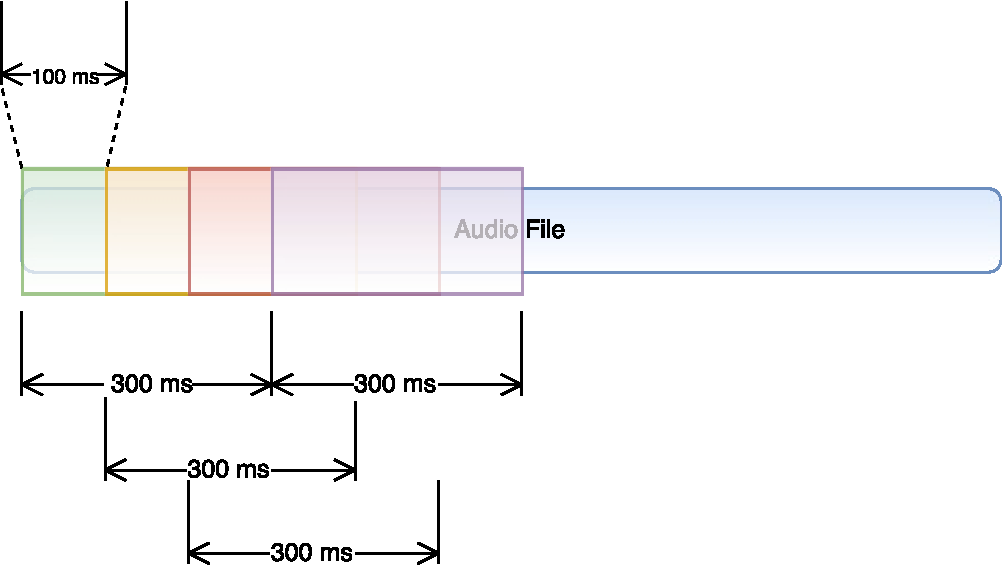
\includegraphics[scale=0.7]{OverlappingSplits300ms.pdf}
    \caption{Overlapping Segmentation}
    \label{fig:overlappingSegmentation}
\end{figure}

\subsection{Re-assembling the segments}
The classifier gave the labels of the overlapping segments. So all we had to do was to remove the segments which were labelled as STUTTER and combine the segments labelled as NORMAL. We took a set difference to get the chunks of audio which contains only NORMAL speech.

One way of assembling the segments was to append contiguous chunks together as show in figure \ref{fig:naiveReassembling} but this will result in sharp interjections at the point of concatenation and will result in very artificial sounding voice.

So instead of na\"ively appending the adjacent chunks, we interpolated the audio samples between the end of the previous chunk and the beginning of the current chunk as shown in figure \ref{fig:smoothedReassembling}.

\begin{figure}[!ht]
    \centering
    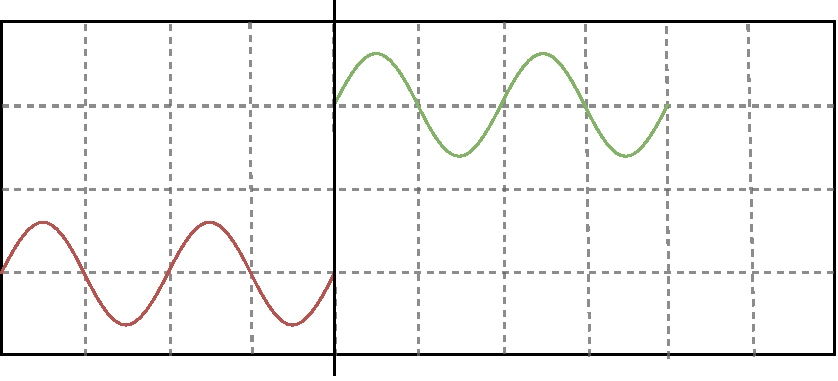
\includegraphics[scale=0.8]{NaiveReassembling.pdf}
    \caption{Na\"ive Re-assembling}
    \label{fig:naiveReassembling}
    
    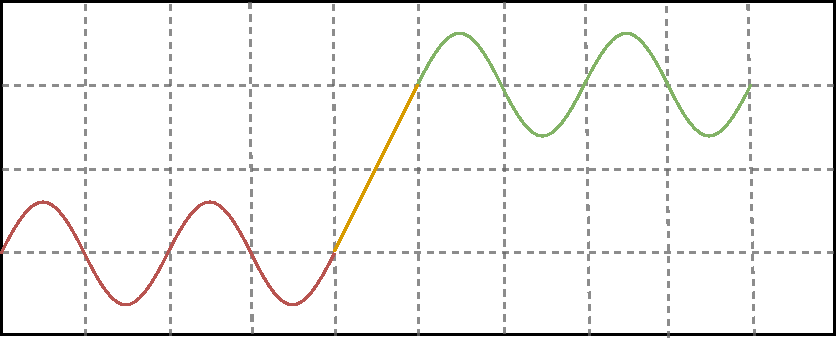
\includegraphics[scale=0.8]{SmoothReassembling.pdf}
    \caption{Smoothed Re-assembling}
    \label{fig:smoothedReassembling}
\end{figure}

The entire audio correction pipeline took 20 sec for an audio of duration 2 min 44 sec. And out of the 20 seconds, $\sim$98\% time \label{correctionDuration} was for feature extraction. Segmentation and classification were instantaneous.

\section{Speech-to-text}
The UCLASS dataset \cite{uclass} is in British English. Instead of training our own Speech-to-text framework on British English, we used the IBM Watson's Speech-to-text \cite{speechToText} which already has a trained model for GB English.

\chapter{Experiments and Results}
As we can see from table \ref{table:werComparision}, our model is far from perfect but we achieved some improvement over the un-modified audio files.

With the limited dataset available for training, we could only achieve this much accuracy.

There were cases where our corrected audio gave even worse WER (M\_0100\_12y3m\_1) but we achieved significant improvement for M\_1017\_11y8m\_1 and M\_1017\_13y2m\_1.

\begin{table}[ht]
\centering
\caption{Comparison of WER of original audio and the corresponding corrected audio}
\label{table:werComparision}
\begin{tabular}{|l|r|r|}
\hline
\textbf{Subject}           & \multicolumn{1}{l|}{\textbf{Original (\%WER)}} & \multicolumn{1}{l|}{\textbf{Corrected (\%WER)}} \\ \hline
\textbf{M\_0017\_19y2m\_1} & 74.928\%                                       & 73.775\%                                        \\ \hline
\textbf{M\_0065\_20y1m\_1} & 125.000\%                                      & 116.429\%                                       \\ \hline
\textbf{M\_0100\_12y3m\_1} & 84.173\%                                       & 89.928\%                                        \\ \hline
\textbf{M\_1017\_11y8m\_1} & 55.396\%                                       & 48.921\%                                        \\ \hline
\textbf{M\_1017\_13y2m\_1} & 59.322\%                                       & 46.610\%                                        \\ \hline
\end{tabular}
\end{table}

\chapter{Summary and Future work}
This study shows that the current state of art speech-to-text systems perform rather poorly with the speech of people having different ability for speech. With a little modification to the speech-to-text pipeline and a considerable amount of dataset, we can achieve a better result for predictions for almost 70 million people worldwide.

As mentioned in \ref{correctionDuration}, around $\sim$98\% time went in feature extraction, we could find some other feature extraction library (currently we are using librosa \cite{librosa}) which can extract feature in less duration or even look at other features which are more representative of stuttered speech.

The source code of the project can be found at \href{https://github.com/anshulgupta0803/stutter-speech-recoginition}{https://github.com/anshulgupta0803/stutter-speech-recoginition}.


\bibliographystyle{plain}
\bibliography{references}
\end{document}
